\subsection{Synthetic study with exact truth}\label{sec:synth}
\paragraph{Design.} The pool has $128$ configurations and $N=20{,}000$ items; the reference cell has $n=200$ tuning items, $K=16$ searched configurations, true-accuracy spread $\tau=0.01$, latent correlation $\rho=0.5$, mean accuracy $0.3$ and best-of-$K$ search. We vary one factor at a time (OFAT, $2000$ whole-pipeline repetitions per cell) and run an $n\times K\times\tau\times$procedure interaction grid ($500$ repetitions per cell) and stress cells ($2000$), $106$ cells in all. The truth of the selected configuration is exact. All gaps are in percentage points (pp) with Monte-Carlo standard errors (s.e.) from the repetitions.

\paragraph{How large is the gap (Q1)?}
In the reference cell the naive report overstates the fresh-item accuracy of the selected configuration by $\N{ref_naive_bias}\pm\N{ref_naive_biasse}$~pp (mean selected true accuracy $\N{ref_mu_sel}\%$), and the naive 95\% Wilson interval covers it in only $\N{ref_naive_cover}\%$ of repetitions (Table~\ref{tab:ref}, Fig.~\ref{fig:reliab} in Appendix~\ref{app:figs}). The gap exists even when all configurations are equally good ($\tau=0$: $\N{gap_tau00}$~pp), so it is a pure selection effect, and it grows with the number of candidates searched ($K=2$: $\N{gap_K2}$~pp; $K=16$: $\N{gap_K16}$~pp; $K=128$: $\N{gap_K128}$~pp) and shrinks with the tuning-set size ($n=50$: $\N{gap_n50}$~pp; $n=2000$: $\N{gap_n2000}$~pp; Figs.~\ref{fig:gap}, \ref{fig:factors}). At the most unfavourable stress cell we ran ($n=50$, $K=128$, accuracy near chance) it is $\N{stress_gap}$~pp and interval coverage drops to $\N{stress_cover}\%$.

\begin{figure}[tbp]
\centering
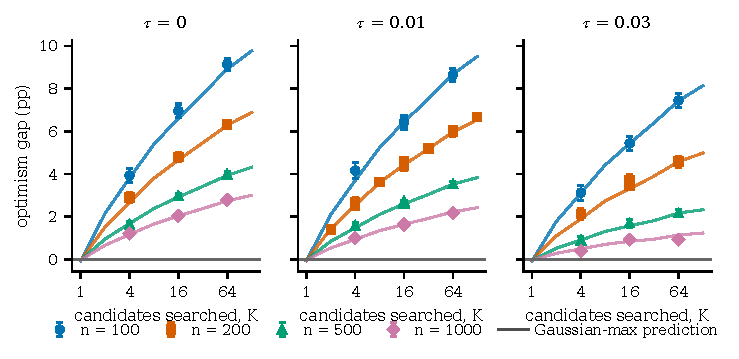
\includegraphics[width=.66\linewidth]{figures/e1_gap_vs_K_rho0.5.pdf}
\caption{Optimism gap (naive report minus exact true accuracy of the selected configuration, pp) for best-of-$K$ search against the number of candidates $K$, per tuning-set size $n$, in three panels by true spread $\tau$ ($\rho=0.5$). Markers: simulation (interaction grid, $500$ repetitions per point), bars $\pm1.96$ Monte-Carlo s.e.; lines: Gaussian-max prediction (Sec.~\ref{sec:method}). $K=1$ has no search and no gap. Over the $\N{th_cells}$ cells with both, observed minus predicted ranges from $\N{th_dmin}$ to $+\N{th_dmax}$~pp; the line extends to $K=128$, where the grid has no simulation.}\label{fig:gap}
\end{figure}

\paragraph{What drives it (Q2).}
Fig.~\ref{fig:factors} varies each factor from the reference cell. The gap is driven mainly by $n$ and $K$. A larger true spread $\tau$ lowers it ($\tau=0.03$: $\N{gap_tau003}$~pp), because a real quality difference makes the selection less noisy. Strong correlation between configurations lowers it ($\rho=0.9$: $\N{gap_rho9}$~pp vs. $\rho=0$: $\N{gap_rho0}$~pp), since correlated candidates share their noise. Generation noise raises it slightly ($\varepsilon=0.2$: $\N{gap_eps2}$~pp) and so does leakage of tuning items into the prompt, which also drives coverage down ($8$ leaked items: gap $\N{gap_leak8}$~pp, naive coverage $\N{cov_leak8}\%$). Among search procedures, successive halving has a smaller gap ($\N{gap_sh}$~pp) than best-of-$K$ and successive rejects ($\N{gap_sr}$~pp); it uses part of the data to eliminate and still reports on all of it, but its coverage is still $\N{cov_sh}\%$. The Gaussian-max prediction agrees with the simulation in the $\N{th_cells}$ cells where both exist (mean absolute difference $\N{th_meanabs}$~pp, at most $\N{th_maxabs}$~pp; $\N{th_rho5_cells}$ cells have $\rho=0.5$, and the largest simulated $K$ is $\N{th_Kmax}$, in one cell). It slightly \emph{under}predicts: the observed gap is larger in $\N{th_above}$ of $\N{th_cells}$ cells (mean difference $+\N{th_meandiff}$~pp; sign test $p\approx\N{th_signp}\times10^{-4}$), and in the $\N{th_nz}$ cells that differ by more than two combined s.e.\ it is larger in $\N{th_nz_above}$ and smaller in $\N{th_nz_below}$. We use it as an approximation, not a theorem.

\begin{figure}[tbp]
\centering
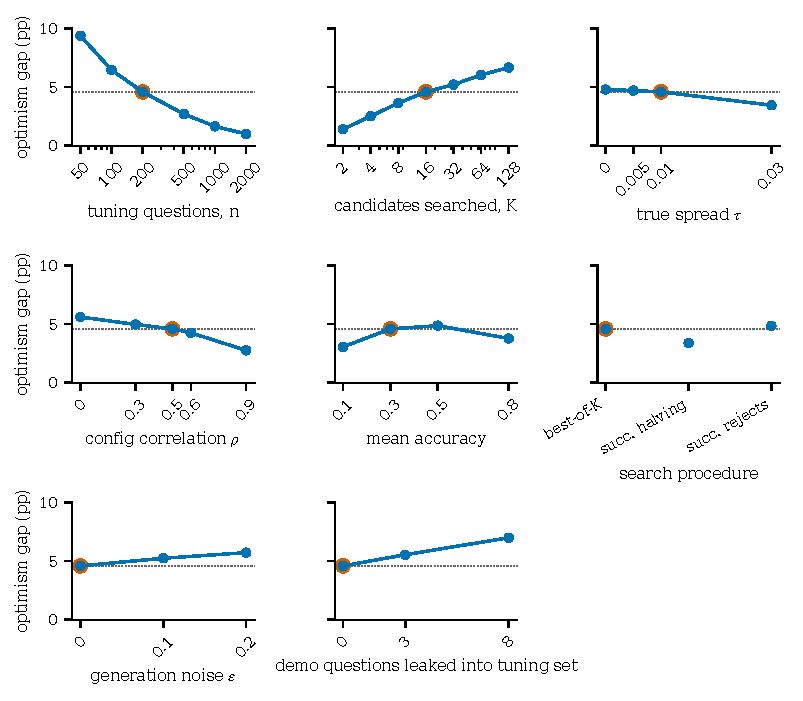
\includegraphics[width=.68\linewidth]{figures/e2_factor_effects.pdf}
\caption{Optimism gap of the naive report when one factor is varied and the others stay at the reference cell ($n=200$, $K=16$, $\tau=0.01$, $\rho=0.5$, mean accuracy $0.3$, best-of-$K$, no generation noise, no leakage; orange ring and dotted line). $2000$ repetitions per point, bars $\pm1.96$ Monte-Carlo s.e. Greedy search ran only at $K=128$ and is not comparable.}\label{fig:factors}
\end{figure}

\paragraph{Does the gap change conclusions (Q3)?}
We ask whether a method licenses the claim ``the tuned system beats the untuned baseline''. The baseline is a fixed pool configuration (index $0$, drawn like the others, chosen independently of the candidates but possibly among them by chance), scored on the same tuning items, or on the report items for the held-out split. A method \emph{claims} when (report $-$ baseline score)$/\mathrm{se}>z$, with $\mathrm{se}$ the paired standard error of the per-item difference between the selected and the baseline configuration and $z=1.645$ (one-sided $5\%$; the simultaneous critical value for the simultaneous bound). The claim is \emph{false} when the selected configuration is in truth not better than the baseline, $\mu_{\hat c}\le\mu_{\text{base}}$, and the false-claim rate is the share of claims among such repetitions ($\N{ref_nonpos}\%$ of the repetitions in the reference cell). Its null value is the boundary rate $5\%$ at $\mu_{\hat c}=\mu_{\text{base}}$; below it the rate should be lower. Requiring a true gain of $0.5$ ($1$)~pp for the claim to count as true changes the naive rate in the reference cell only to $\N{mg_naive_le05}\%$ ($\N{mg_naive_le1}\%$), and a claim with a negative true difference occurs in $\N{mg_naive_ws}\%$ of all repetitions (split: $\N{mg_split_ws}\%$, simultaneous: $\N{mg_simul_ws}\%$). A \emph{false ship} (Table~\ref{tab:ref}) is a report at least $2$~pp above the baseline's true score while the selected configuration's true score is below that bar. In the reference cell the naive report claims in $\N{ref_naive_claim}\%$ of all repetitions and in $\N{ref_naive_fp}\%$ of the false cases, against the boundary rate of $5\%$ (Fig.~\ref{fig:claims}a). With $K=128$ it does in $\N{fp_K128}\%$. The comparison of two tuned systems is equally affected when their search budgets differ (Fig.~\ref{fig:claims}b): at $\tau=0$, i.e.\ identical systems, a system tuned over $64$ configurations is claimed to beat one with a single configuration in $\N{cmp_00_6401_claim}\%$ of $\N{cmp_reps}$ repetitions, and the claim is also not true (true difference not positive) in $\N{cmp_00_6401_false}\%$ ($\N{cmp_00_6401_fc05}\%$ if a true gain of $0.5$~pp is required); the average reported difference is $\N{cmp_00_6401_diff}$~pp against a true one of about zero. With equal budgets ($16$ vs.\ $16$) the false-claim rate is $\N{cmp_00_1616_false}\%$ at $n=200$: the bias cancels when both systems were searched alike, and does not when they were not.

\begin{figure}[tbp]
\centering
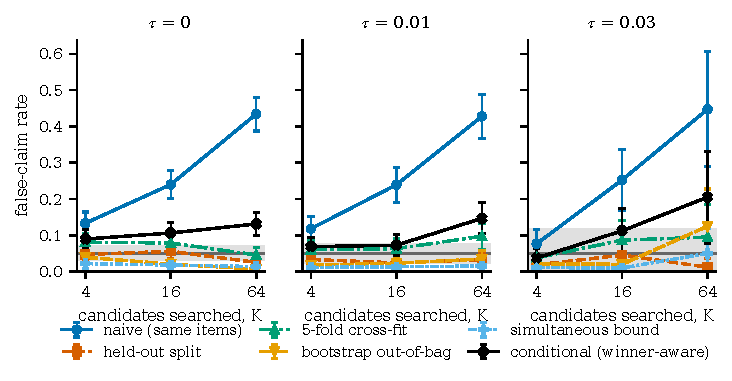
\includegraphics[width=.68\linewidth]{figures/e4_false_claims_argmax_rho0.5_n200.pdf}\\[2pt]
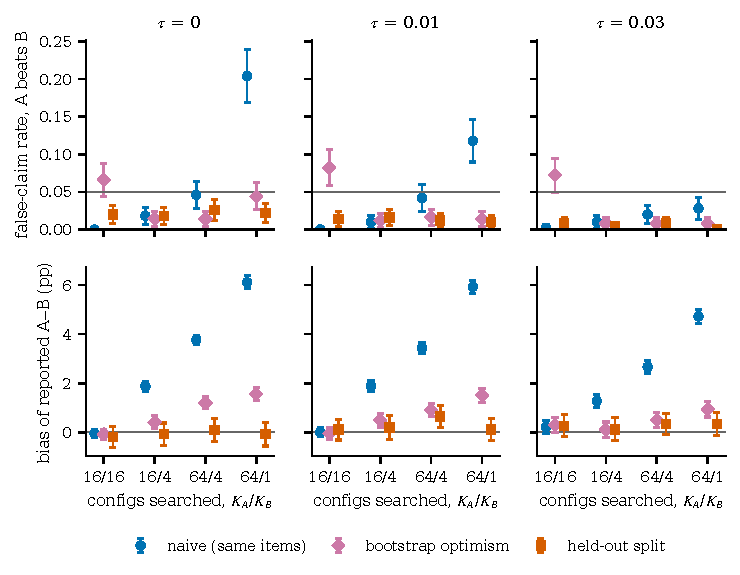
\includegraphics[width=.68\linewidth]{figures/e4_unequal_budget_n200.pdf}
\caption{(a) Share of repetitions in which a method licenses ``tuned beats untuned baseline'' (one-sided 5\%) among those where the selected configuration is truly not better ($n=200$, $\rho=0.5$, best-of-$K$; $500$ repetitions, bars $\pm1.96\sqrt{p(1-p)/m}$ with $m$ the repetitions in the denominator; the grey band is the binomial 95\% band around the nominal $0.05$). (b) Two systems tuned with $K_A$ and $K_B$ configurations, $n=200$, $500$ repetitions. Top: share of repetitions claiming ``$A$ beats $B$'' while $A$ is truly not better; line: nominal $0.05$. Bottom: bias of the reported $A-B$ difference (pp), bars $\pm1.96$ s.e.}\label{fig:claims}
\end{figure}

\paragraph{Reporting methods (Q4, Q5).}
Table~\ref{tab:ref} (Appendix~\ref{app:more}) and Fig.~\ref{fig:reliab} (Appendix~\ref{app:figs}) give bias, coverage and width in the reference cell. The study plan, written before the runs, fixes a reliability criterion that we apply to all $106$ cells and every method: $|$bias$|\le\max(2\,\text{s.e.},0.5~\text{pp})$ and 95\% coverage inside the binomial Monte-Carlo band around $0.95$. The coverage condition is two-sided, so a conservative interval fails it; we therefore also count under-coverage (below the band) and over-coverage (above it). The held-out split meets the criterion in $\N{rel_split_ok}$ of $\N{rel_split_cells}$ cells; its $\N{split_fail_bias}$ bias and $\N{split_fail_cov}$ coverage failures ($\N{rel_split_under}$ under, $\N{rel_split_over}$ over; largest $|$bias$|$ $\N{split_maxabsbias}$~pp) are of the size expected from testing $106$ cells twice at the 5\% level. It pays with half of the items (width $\N{ref_split_width}$ vs.\ $\N{ref_naive_width}$~pp; RMSE $\N{ref_split_rmse}$ vs.\ $\N{ref_naive_rmse}$~pp in the reference cell) and reports the configuration chosen from $n/2$ items, so we compare protocols at equal total items below. The naive report meets the criterion in only $\N{rel_naive_ok}$ of $106$ cells, under-covering in $\N{rel_naive_under}$. The simultaneous bound keeps the naive bias ($\N{ref_simul_bias}$~pp) but under-covers in only $\N{rel_simul_under}$ cells and over-covers in $\N{rel_simul_over}$ ($\N{ref_simul_cover}\%$ in the reference cell, width $\N{ref_simul_width}$~pp): valid and conservative. Five-fold cross-fitting under-covers in $\N{rel_crossfit_under}$ cells; the bootstrap corrections reduce the bias (out-of-bag: $\N{ref_boot_oob_bias}$~pp in the reference cell) but mostly over-cover ($\N{rel_boot_oob_over}$ over, $\N{rel_boot_oob_under}$ under), so they meet the full criterion in only $\N{rel_boot_oob_ok}$ cells. Our implementations of winner-aware conditional inference and of a hybrid interval (Appendix~\ref{app:defs}) agree with a closed form ($K=2$) and with a port of the authors' replication code, and are calibrated in exact Gaussian cases (coverage $\N{val_cov_min}$--$\N{val_cov_max}\%$). The conditional interval is nonetheless very wide in the reference cell (width $\N{ref_cond_width}$~pp; RMSE of its median $\N{ref_cond_rmse}$~pp) because the winner's lead over the truncation boundary is below $0.5$ standard errors in $\N{val_ref_lead_lt05}\%$ of repetitions. The hybrid has coverage $\N{hy_hybrid_covmin}$--$\N{hy_hybrid_covmax}\%$ at width $\N{hy_hybrid_width}$~pp ($\N{hy_simul_width}$~pp for the simultaneous bound) in the region we ran ($\rho=0.5$, mean accuracy $0.3$, $K\le64$, $\N{hy_cells}$ cells), but its point estimate is no better than the naive one. The Ladder-type report \citep{blum2015ladder} reduces the naive bias but does not remove it ($\tau=0$, $n=200$, $K=16$: $\N{lad_ladder_K16_bias}$ vs.\ $\N{lad_naive_K16_bias}$~pp).

\paragraph{Reporting protocols at equal item budgets (Q5).}
We score every protocol against the true accuracy of the configuration \emph{it} ships, at equal total items (Table~\ref{tab:fresh} in Appendix~\ref{app:more}; $\N{fr_ncells}$ combinations of $\tau\in\{0,.01,.03\}$, $K\in\{4,16,64\}$, $\rho\in\{.5,.9\}$ and $200$ or $400$ items, $\N{fr_reps}$ repetitions). A \emph{fresh-set} protocol tunes on $n_{\text{tune}}$ items, ships the winner and reports its accuracy on $m$ new items. In the reference cell with $200$ items in all, the $100/100$ fresh-set report and the $50/50$ split are unbiased ($\N{fr_fresh100_200_bias}$ and $\N{fr_split_200_bias}$~pp) with $95\%$ coverage, but their RMSE is $\N{fr_fresh100_200_rmse}$ and $\N{fr_split_200_rmse}$~pp because the report items carry their own sampling error; the best fresh allocation ($50/150$) has RMSE $\N{fr_fresh50_200_rmse}$~pp; the out-of-bag bootstrap on all $200$ items has bias $\N{fr_boot_oob_200_bias}$~pp, RMSE $\N{fr_boot_oob_200_rmse}$~pp and coverage $\N{fr_boot_oob_200_cover}\%$, the naive report $+\N{fr_naive_200_bias}$~pp and $\N{fr_naive_200_rmse}$~pp. The out-of-bag bootstrap has the smaller RMSE than the split and than the half-and-half fresh set in all $\N{fr_ncells}$ combinations, with coverage $\N{fr_oob_covmin}$--$\N{fr_oob_covmax}\%$ (conservative in most), while the hybrid's RMSE exceeds the naive one in $\N{fr_hyb_gt_naive}$. Holding items out thus buys an unbiased, assumption-free report, not a more accurate one. The out-of-bag bootstrap needs the per-item outcomes of every searched candidate and a search that can be replayed on resampled items; we checked it only for the searches here.

\paragraph{Ranking several tuned systems.}
For five systems tuned on the same items with $4$, $8$, $16$, $32$ and $64$ configurations at $\tau=0$ (all equally good, $n=200$, $\N{rk_reps}$ repetitions; Fig.~\ref{fig:rank} in Appendix~\ref{app:figs}), the naive report puts the largest-budget system first in $\N{rk_naive_big_rep}\%$ of repetitions, whereas it is truly best in $\N{rk_naive_big_true}\%$ (the held-out split: $\N{rk_split_big_rep}\%$ vs.\ $\N{rk_split_big_true}\%$); with five systems tuned alike ($16$ configurations each) the naive rate is $\N{rk_naive_eq_big_rep}\%$. When quality differs ($\tau=0.03$) the naive rank correlation with the truth is not worse than the split's (Kendall's $\tau_b$ $\N{rk_naive_kt_uneq}$ vs.\ $\N{rk_split_kt_uneq}$); the distortion is that the budget, not the quality, orders equally good systems. At an equal total budget of $400$ items the out-of-bag bootstrap, the split and the half-and-half fresh set put the $64$-candidate system first in $\N{rkb_oob_big_rep}$, $\N{rkb_split_big_rep}$ and $\N{rkb_fresh_big_rep}\%$ of repetitions at $\tau=0$ ($\N{rkb_naive_big_rep}\%$ for the naive report; truly best in $\N{rkb_big_true}\%$), so they remove the budget effect, but with true differences ($\tau=0.03$) none ranks better than the naive report by Kendall's $\tau_b$ ($\N{rkb_oob_kt}$, $\N{rkb_split_kt}$, $\N{rkb_fresh_kt}$ vs.\ $\N{rkb_naive_kt}$; $\N{rkb_reps}$ repetitions).




\subsection{Real LLM on MMLU-Pro}\label{sec:real}
\paragraph{Scale reached.} The pool is all $K=\N{real_K}$ configurations of a factorial grid of instruction wording, demonstration set and option layout, each scored on all $\N{real_items}$ items by Qwen2.5-0.5B-Instruct. Their accuracies are $\N{real_accmin}$--$\N{real_accmax}\%$ (mean $\N{real_accmean}\%$; chance $10\%$), a spread of $\N{real_sd}$~pp (s.d.), with a mean item-level correlation of $\N{real_corr}$ between configurations. This is a small-spread regime with one small model; it is not a study of large $K$, of stronger models or of DSPy or MIPRO, which we did not run. Searches are replayed on the cached $0/1$ matrix ($\N{real_reps}$ repetitions per cell). In the \emph{disjoint} arm ($n\le400$) the tuning items are drawn without replacement and the truth is the selected configuration's accuracy on the remaining $2000-n$ items; in the \emph{i.i.d.} arm they are drawn with replacement and the truth is the accuracy over the whole pool ($n\le\N{real_iid_nmax}$).

\paragraph{The gap is present and has the same shape.} With exhaustive search over the $K=\N{real_K}$ configurations the naive report exceeds the held-out accuracy of the selected configuration by $\N{real_gap_n50}\pm\N{real_gapse_n50}$~pp at $n=50$, $\N{real_gap_n100}$ at $n=100$, $\N{real_gap_n200}\pm\N{real_gapse_n200}$ at $n=200$ and $\N{real_gap_n400}$~pp at $n=400$, and the i.i.d.\ arm gives the same ($\N{real_iid_gap_n50}$, $\N{real_iid_gap_n200}$, $\N{real_iid_gap_n400}$~pp; Fig.~\ref{fig:real}). At $n=200$ it grows with the number of candidates ($K=1$: $\N{real_gap_K1_n200}\pm\N{real_gapse_K1_n200}$, $K=2$: $\N{real_gap_K2_n200}$, $K=4$: $\N{real_gap_K4_n200}$, $K=\N{real_K}$: $\N{real_gap_n200}$~pp), although the search has little to find (mean regret $\N{real_regret_n200}$~pp). At $n=200$ the cheaper searches shrink the gap but do not remove it: successive halving $\N{real_gap_sh}$~pp, greedy coordinate search over the factorial grid $\N{real_gap_greedy}$~pp, successive rejects $\N{real_gap_sr}$~pp, against $\N{real_gap_n200}$~pp for exhaustive search. The naive Wilson interval covers the truth in only $\N{real_cover_n200}\%$ of repetitions at $n=200$ ($\N{real_cover_n50}\%$ at $n=50$), and the naive report licenses ``tuned beats the baseline'' in $\N{real_fp_n200}\%$ of the repetitions at $n=200$ in which the selected configuration is truly no better ($\N{real_fp_n50}\%$ at $n=50$; nominal $5\%$).

\paragraph{The Gaussian-maximum formula and the generator, checked on the real matrix.} Fed with the empirical covariance of the real matrix, the formula of Sec.~\ref{sec:method} predicts the replayed gap at $K=\N{real_K}$ as $\N{gm_pred_n50}$ vs.\ $\N{gm_rep_n50}$~pp ($n=50$), $\N{gm_pred_n200}$ vs.\ $\N{gm_rep_n200}$ ($200$) and $\N{gm_pred_n400}$ vs.\ $\N{gm_rep_n400}$~pp ($400$; Fig.~\ref{fig:real}a); over all $\N{gm_cells}$ cells ($K\le\N{real_K}$, $n$ up to $\N{gm_nmax}$, both arms) the difference is at most $\N{gm_maxdiff}$~pp, with $\N{gm_z2}$ cells beyond two Monte-Carlo s.e. Generator settings matched to the real accuracies, mean item correlation (latent $\rho=\N{gen_rho}$) or the full pairwise correlations reproduce the real naive gap to within about ten percent (one-$\rho$ copula $\N{gen_uni_rel}\%$ on average, pairwise copula $\N{gen_tet_rel}\%$ for $K\ge4$), not exactly (Appendix~\ref{app:calib}).

\begin{figure}[tbp]
\centering
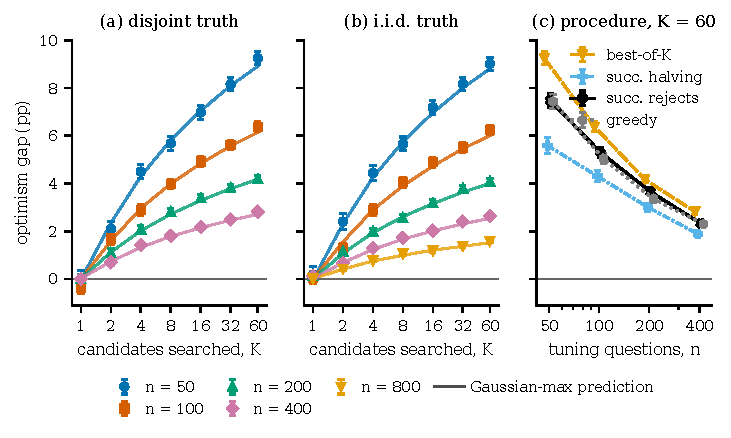
\includegraphics[width=.68\linewidth]{figures/e3_real_gap.pdf}
\caption{Real setting (Qwen2.5-0.5B-Instruct, MMLU-Pro, $K\le\N{real_K}$ complete configurations, $\N{real_reps}$ repetitions per point, bars $\pm1.96$ Monte-Carlo s.e.). Optimism gap of the naive report of best-of-$K$ search against the number of candidates searched, one colour per tuning-set size $n$; markers are the replay, lines the Gaussian-maximum prediction from the empirical covariance of the real matrix; $K=1$ is the no-search control. (a) Disjoint truth arm. (b) I.i.d.\ truth arm (truth over the whole pool). (c) At $K=\N{real_K}$, best-of-$K$, successive halving, successive rejects and greedy coordinate search against $n$ (disjoint arm).}\label{fig:real}
\end{figure}

\paragraph{Reporting methods.} Table~\ref{tab:real} (Appendix~\ref{app:more}) gives the real-setting version of the reference table. At $n=200$ the held-out split is unbiased ($\N{real_split_n200_bias}\pm\N{real_split_n200_biasse}$~pp, coverage $\N{real_split_n200_cover}\%$), the out-of-bag bootstrap reduces the bias to $\N{real_boot_oob_n200_bias}$~pp at nearly the naive width, the hybrid interval covers $\N{real_hybrid_n200_cover}\%$ with RMSE $\N{real_hybrid_n200_rmse}$~pp (naive $\N{real_naive_n200_rmse}$) and the conditional interval, $\N{real_cond_n200_width}$~pp wide, covers $\N{real_cond_n200_cover}\%$. At equal total items ($200$; Table~\ref{tab:freshreal}) the RMSE is $\N{frr_boot_oob_200_rmse}$~pp for the out-of-bag bootstrap (coverage $\N{frr_boot_oob_200_cover}\%$), $\N{frr_fresh50_200_rmse}$ and $\N{frr_fresh100_200_rmse}$~pp for $50$/$150$ and $100$/$100$ tuning/fresh items, $\N{frr_split_200_rmse}$~pp for the split and $\N{frr_naive_200_rmse}$~pp for the naive report: the order of the synthetic study.
